\documentclass[12pt,a4paper]{article}

% ============================================================
% Pacotes
% ============================================================
\usepackage[portuguese]{babel}
\usepackage[utf8]{inputenc}
\usepackage[T1]{fontenc}
\usepackage[a4paper, margin=2.5cm, top=2.8cm, bottom=2.8cm]{geometry}
\usepackage{graphicx}
\usepackage[colorlinks=true, linkcolor=black, citecolor=blue, urlcolor=blue]{hyperref}
\usepackage{booktabs}
\usepackage{array}
\usepackage{float}
\usepackage{caption}
\usepackage{subcaption}
\usepackage{amsmath}
\usepackage{fancyhdr}
\setlength{\headheight}{15pt}
\usepackage{enumitem}
\usepackage{xcolor}
\usepackage{tabularx}
\usepackage{microtype}
\usepackage{parskip}

% ============================================================
% Caminho das imagens
% ============================================================
\graphicspath{{./}{../}{../validade_predictions/}{../dados_exames/}}

% ============================================================
% Cabeçalho e rodapé
% ============================================================
\pagestyle{fancy}
\fancyhf{}
\fancyhead[L]{\small MediaTrix}
\fancyhead[R]{\small Projeto Integrador --- L.EIC}
\fancyfoot[C]{\thepage}
\renewcommand{\headrulewidth}{0.4pt}

% ============================================================
% Início do documento
% ============================================================
\begin{document}

% ============================================================
% FOLHA DE ROSTO
% ============================================================
\begin{titlepage}
  \thispagestyle{empty}
  \begin{center}
    \textbf{\Large Faculdade de Engenharia da Universidade do Porto} \\
    \large Licenciatura em Engenharia Informática e Computação\\
    \vspace{2.5cm}

    {\LARGE Relatório Final de Projeto Integrador \\}
    \vspace{0.2cm}
    {\LARGE \textbf{MediaTrix: Plataforma Web de Previsão de Médias de Acesso ao Ensino Superior Português} \\}
    \vspace{1cm}
    {\large José Torres - up202307047 \\ José Reis - up202307304 \\ Tiago Yin - up202306438 \\ Vicente Silva - up202303702}

    \vspace{0.8cm}
    {\large U.Porto --- L.EIC --- Projeto Integrador}

    \vspace{0.4cm}
    {\large Junho de 2026}

    \vfill
    \vspace{0.5cm}
    
\includegraphics[height=0.1\textwidth]{feup_logo.png}
  \end{center}
\end{titlepage}

% ============================================================
% ÍNDICE
% ============================================================
\tableofcontents
\newpage

% ============================================================
% 1. INTRODUÇÃO
% ============================================================
\section{Introdução}

\subsection{Objetivo do Relatório}

O presente relatório documenta o trabalho realizado no âmbito da unidade curricular de Projeto Integrador (PI) da Licenciatura em Engenharia Informática e Computação (L.EIC) da Faculdade de Engenharia da Universidade do Porto (FEUP). O objetivo é descrever o processo de desenvolvimento, as decisões técnicas e os resultados obtidos na conceção e implementação do projeto MediaTrix, demonstrando o cumprimento dos objetivos de aprendizagem da UC.

\subsection{Contexto Organizacional}

O projeto foi desenvolvido no contexto académico da FEUP, como aplicação de competências em engenharia de software, ciência de dados e desenvolvimento web, por uma equipa de quatro estudantes da L.EIC. Não existiu empresa ou instituição de acolhimento externa; o projeto foi inteiramente concebido, planeado e executado pela equipa, com orientação do Prof.\ Carlos Baquero (FEUP/DEI).

\subsection{Problema e Motivação}

Em Portugal, o acesso ao ensino superior público é regulado pela Direção-Geral do Ensino Superior (DGES), que todos os anos divulga as notas mínimas de entrada em cada par curso--instituição para três fases de candidatura. Estas notas, designadas \textit{médias de acesso} ou \textit{notas de entrada}, são determinantes para as decisões de candidatura dos estudantes do ensino secundário.

No entanto, as notas de acesso variam anualmente em função do número de candidatos, dos resultados dos exames nacionais, das vagas disponíveis e das preferências agregadas dos candidatos. Esta imprevisibilidade gera incerteza significativa: um estudante que planeia candidatar-se em 2026 não sabe com precisão qual será a nota mínima exigida. As ferramentas existentes limitam-se a apresentar dados históricos sem qualquer componente preditiva ou de simulação da candidatura.

A motivação para o MediaTrix nasce precisamente desta lacuna: criar uma plataforma que, com base em dados históricos oficiais e modelos estatísticos e computacionais, forneça previsões fundamentadas das notas de acesso para o ano seguinte, bem como ferramentas que permitam ao candidato simular a sua própria candidatura e estimar a probabilidade de ser colocado.

\subsection{Objetivos do Trabalho e Resultados Esperados}

Os objetivos principais do projeto foram:
\begin{enumerate}[noitemsep]
  \item Recolher e estruturar dados oficiais da DGES referentes aos anos de 2017 a 2025.
  \item Desenvolver um motor de simulação do processo de candidatura ao ensino superior, replicando a lógica do algoritmo de \textit{matching} da DGES.
  \item Treinar um modelo de inteligência artificial para calibrar o comportamento de preferência dos candidatos com base em dados históricos.
  \item Implementar um algoritmo de previsão de notas de acesso com intervalos de confiança de 95\%.
  \item Desenvolver uma plataforma web acessível e intuitiva para consulta de dados históricos, previsões e simulação de candidatura.
\end{enumerate}

O resultado esperado era uma aplicação web funcional, capaz de apresentar previsões com erro médio inferior a 10 pontos (escala 0--200) e um simulador de candidatura que calculasse corretamente a nota do utilizador de acordo com a fórmula oficial de cada curso.

\subsection{Estrutura do Relatório}

A Secção~\ref{sec:metodologia} descreve a metodologia de desenvolvimento e as principais atividades realizadas. A Secção~\ref{sec:solucao} apresenta os requisitos, a arquitetura técnica e a solução desenvolvida, incluindo os resultados de validação. A Secção~\ref{sec:conclusoes} sumariza os resultados alcançados, as lições aprendidas e o trabalho futuro.

% ============================================================
% 2. METODOLOGIA
% ============================================================
\section{Metodologia Utilizada e Principais Atividades Desenvolvidas}
\label{sec:metodologia}

\subsection{Metodologia de Desenvolvimento}

O projeto seguiu uma metodologia de desenvolvimento iterativo e incremental, organizada em ciclos com entregas progressivas. Não foram seguidas cerimónias formais de \textit{Scrum}, optando-se por uma abordagem baseada em marcos de entrega (\textit{milestones}) com revisão contínua e reuniões periódicas de equipa. O controlo de versões foi gerido com \textbf{Git}, com repositório alojado em \textbf{GitHub}. O desenvolvimento do \textit{frontend} utilizou \textbf{Vite} como servidor de desenvolvimento, com \textit{hot module replacement} (HMR) para ciclos de \textit{feedback} rápidos. Os módulos Python foram desenvolvidos e testados localmente, com os dados processados guardados em ficheiros JSON e CSV.

\subsection{Intervenientes, Papéis e Responsabilidades}

A equipa foi composta por quatro elementos, com orientação do \textbf{Prof.\ Carlos Baquero} (FEUP/DEI). Os papéis e responsabilidades principais foram distribuídos da seguinte forma:

\begin{itemize}[noitemsep]
  \item \textbf{José Torres} (up202307047): 
  \item \textbf{José Reis} (up202307304):
  \item \textbf{Tiago Yin} (up202306438): 
  \item \textbf{Vicente Silva} (up202303702):
\end{itemize}

Os principais \textit{stakeholders} identificados foram:

\begin{itemize}[noitemsep]
  \item \textbf{Candidatos ao ensino superior}: utilizadores primários da plataforma, com necessidade de informação clara e previsões fiáveis para apoiar as suas decisões de candidatura.
  \item \textbf{Encarregados de educação}: utilizadores secundários, interessados em apoiar as decisões dos candidatos.
  \item \textbf{DGES}: entidade responsável pelos dados oficiais que constituem a base de todo o sistema, embora sem interação direta no projeto.
\end{itemize}

\subsection{Atividades Desenvolvidas}

O desenvolvimento decorreu ao longo do segundo semestre do ano letivo 2025/2026 e pode ser dividido nas fases descritas na Tabela~\ref{tab:fases}.

\begin{table}[H]
\centering
\caption{Fases de desenvolvimento do projeto MediaTrix.}
\label{tab:fases}
\begin{tabularx}{\textwidth}{llX}
\toprule
\textbf{Fase} & \textbf{Duração} & \textbf{Atividades Principais} \\
\midrule
1 --- Análise e Dados & 3 semanas & Recolha dos dados DGES (2017--2025), estruturação dos ficheiros JSON, análise exploratória, definição de requisitos. \\
2 --- Motor de Simulação & 4 semanas & Implementação do gerador de populações e do simulador Gale-Shapley; primeiros testes de validação. \\
3 --- Modelo de IA & 2 semanas & Implementação do módulo de treino com \textit{backpropagation} e \textit{momentum}; calibração de hiperparâmetros; treino 2017--2024. \\
4 --- \textit{Frontend} & 5 semanas & Arquitetura React; implementação dos componentes; integração dos dados; visualizações com Recharts. \\
5 --- Previsão e IC & 2 semanas & Algoritmo de suavização exponencial com reversão à média; cálculo de intervalos de confiança de 95\%. \\
6 --- Validação & 2 semanas & \textit{Backtesting} do algoritmo de previsão; análise de erros; ajuste de parâmetros; melhorias de usabilidade. \\
7 --- Documentação & 1 semana & Elaboração do relatório final. \\
\bottomrule
\end{tabularx}
\end{table}

As principais entregas (\textit{deliverables}) foram:

\begin{itemize}[noitemsep]
  \item \textbf{Conjunto de dados estruturado}: ficheiros JSON com dados de todos os cursos do ensino superior português (2017--2025), incluindo notas de acesso por fase, vagas iniciais e informações de exames de ingresso.
  \item \textbf{Pipeline de simulação}: três módulos Python --- geração de populações sintéticas, simulação do processo de candidatura (Gale-Shapley) e treino do modelo de IA por \textit{online learning}.
  \item \textbf{Pesos neurais treinados}: ficheiro \texttt{pesos\_cursos.json} com os pesos de atratividade de cada curso, resultado de 9 anos de treino incremental.
  \item \textbf{Plataforma web MediaTrix}: aplicação web completa com pesquisa de cursos, visualização histórica, previsões e simulador de candidatura.
\end{itemize}

% ============================================================
% 3. DESENVOLVIMENTO DA SOLUÇÃO
% ============================================================
\section{Desenvolvimento da Solução}
\label{sec:solucao}

\subsection{Requisitos e Restrições}

\subsubsection{Requisitos Funcionais}

\begin{enumerate}[noitemsep]
  \item O sistema deve permitir a pesquisa de cursos por nome, instituição e/ou distrito.
  \item O sistema deve apresentar a evolução histórica das notas de acesso (1.ª, 2.ª e 3.ª fases) de 2017 a 2025 para cada curso.
  \item O sistema deve apresentar previsões de notas de acesso para os 3 anos seguintes com intervalos de confiança de 95\%.
  \item O sistema deve indicar os exames de ingresso obrigatórios e a fórmula de cálculo da nota de candidatura para cada curso.
  \item O sistema deve disponibilizar um simulador que calcule a nota de candidatura do utilizador e a compare com as previsões por fase.
  \item O sistema deve apresentar a distribuição histórica de notas dos exames nacionais relevantes.
  \item O sistema deve ser acessível em dispositivos \textit{desktop} e \textit{mobile} (design responsivo).
\end{enumerate}

\subsubsection{Requisitos Não Funcionais}

\begin{itemize}[noitemsep]
  \item \textbf{Desempenho}: os dados devem ser carregados em menos de 2 segundos numa ligação de banda larga típica.
  \item \textbf{Escalabilidade}: a adição de novos anos de dados não deve requerer alterações à arquitetura da aplicação.
  \item \textbf{Manutenibilidade}: os ficheiros de dados DGES devem poder ser atualizados anualmente sem alterações ao código-fonte.
  \item \textbf{Transparência}: o modelo preditivo e as suas limitações devem estar claramente documentados na interface.
\end{itemize}

\subsubsection{Restrições}

\begin{itemize}[noitemsep]
  \item Os dados de candidatura estão disponíveis publicamente apenas para os anos 2017--2025, limitando a profundidade histórica do modelo.
  \item A DGES não disponibiliza uma API oficial, pelo que a recolha de dados foi feita manualmente a partir dos relatórios publicados.
  \item O sistema é puramente estatístico e não tem acesso a informação sobre o número futuro de candidatos nem sobre os resultados dos exames nacionais do ano de previsão.
\end{itemize}

\subsection{Arquitetura e Tecnologias}

A solução está organizada em dois subsistemas principais: o \textbf{pipeline de dados e treino} (Python) e a \textbf{plataforma web} (React/TypeScript). A Tabela~\ref{tab:arquitetura} apresenta os módulos do sistema e as respetivas responsabilidades.

\begin{table}[H]
\centering
\caption{Módulos do sistema MediaTrix.}
\label{tab:arquitetura}
\begin{tabularx}{\textwidth}{llX}
\toprule
\textbf{Módulo} & \textbf{Tecnologia} & \textbf{Responsabilidade} \\
\midrule
\texttt{gerador\_populacao.py} & Python/NumPy & Geração de populações sintéticas de candidatos (75\,000/ano). \\
\texttt{simulador\_dges.py} & Python/pandas & Simulação do processo de \textit{matching} (Gale-Shapley) com 3 fases. \\
\texttt{treinador\_ia.py} & Python & \textit{Online learning} com \textit{backpropagation} e \textit{momentum} para calibração dos pesos. \\
Frontend (React) & React 19/TypeScript & Interface web: pesquisa, gráficos, simulador de candidatura. \\
\texttt{examDataService.ts} & TypeScript & Carregamento, \textit{parsing} e processamento dos dados JSON; algoritmo de previsão. \\
Dados JSON & --- & Dados DGES 2017--2025, detalhes de cursos, médias de exames, distribuições. \\
\bottomrule
\end{tabularx}
\end{table}

\subsubsection{Pipeline de Dados e Treino}

O pipeline de dados é composto por três módulos Python desenvolvidos de raiz.

\paragraph{Módulo de Geração Sintética (\texttt{gerador\_populacao.py})}

Para simular o processo de candidatura, é necessário modelar uma população de candidatos com características realistas. Este módulo gera anualmente cerca de 75\,000 candidatos sintéticos com base em:

\begin{itemize}[noitemsep]
  \item \textbf{Distribuição de áreas de estudo}: as percentagens de alunos por área científica (Ciências/Saúde, Engenharias, Economia, Humanidades, Artes) seguem os dados publicados pelo Ministério da Educação (DGEEC~\cite{dgeec}).
  \item \textbf{Geolocalização}: o distrito de residência é atribuído com base nos censos populacionais, sendo relevante para a modelação de preferências geográficas.
  \item \textbf{DNA académico} (Percentil Beta): para garantir correlações positivas entre disciplinas afins (por exemplo, um bom aluno a Matemática tende a ser bom a Física), é atribuído a cada aluno um percentil de desempenho base segundo uma distribuição Beta. As notas dos exames nacionais são derivadas deste percentil.
  \item \textbf{Nota interna}: calculada com uma curva de Gauss sobre a média dos exames, refletindo a inflação característica do ensino secundário português.
\end{itemize}

\paragraph{Motor de Simulação e \textit{Matching} (\texttt{simulador\_dges.py})}

Este módulo replica computacionalmente o processo de colocação da DGES, que segue uma variante do algoritmo Gale-Shapley~\cite{gale1962college}:

\begin{itemize}
  \item \textbf{Estrutura de fases}: simula as 3 fases reais de acesso. Na Fase~1, 96\% dos candidatos entram no mercado. As Fases~2 e~3 absorvem as vagas sobrantes e são disputadas por candidatos não colocados e por candidatos \textit{inconformados} --- alunos colocados que tentam mudar de curso apenas quando a sua nota é manifestamente superior ao mínimo do curso onde foram colocados.

  \item \textbf{Construção da ficha de candidatura}: a lista de até 6 opções de cada candidato é construída com um modelo de preferência dinâmico que pondera: (i)~a \textit{atratividade dinâmica} do curso (prestígio histórico ponderado pelos pesos neurais da IA); (ii)~uma \textit{penalização exponencial} que impede candidatos com notas elevadas de colocar como opção cursos muito abaixo do seu nível (``turismo de génios''); e (iii)~um \textit{filtro de dignidade} que expurga cursos com score de interesse nulo da ficha.

  \item \textbf{Algoritmo de colocação}: o algoritmo Gale-Shapley garante que todos os candidatos concorrem em simultâneo. As faculdades retêm os melhores candidatos e rejeitam os restantes, que ``caem'' para a opção seguinte, despoletando um efeito dominó até à estabilização matemática.
\end{itemize}

\paragraph{Treinador de Inteligência Artificial (\texttt{treinador\_ia.py})}

O módulo de treino implementa \textit{online learning} com \textit{backpropagation} e \textit{momentum}, percorrendo os dados cronologicamente de 2017 a 2025. Para cada ano, o erro entre a nota simulada e a nota real da DGES é calculado e usado para ajustar os pesos neurais (\textit{magnetismo}) de cada curso:

\begin{equation}
v_{\text{novo}} = \beta \cdot v_{\text{atual}} + \alpha \cdot \varepsilon_{\text{controlado}}
\label{eq:momentum}
\end{equation}
\begin{equation}
\text{Peso}_{\text{novo}} = \text{Peso}_{\text{atual}} - v_{\text{novo}}
\label{eq:update}
\end{equation}

onde $\alpha = 0.008$ é a \textit{learning rate}, $\beta = 0.5$ é o \textit{momentum}, e $\varepsilon_{\text{controlado}}$ é o erro com \textit{gradient clipping} ($|\varepsilon| \leq 15$). A velocidade é também limitada ($|v| \leq 0.15$) para evitar alterações bruscas causadas por anomalias de um único ano (por exemplo, a pandemia de COVID-19 em 2020). Os pesos resultantes, guardados em \texttt{pesos\_cursos.json}, representam o ``DNA de atratividade'' acumulado de cada curso ao longo de 9 anos.

\subsubsection{Plataforma Web}

A plataforma foi desenvolvida com \textbf{React~19} e \textbf{TypeScript}, usando \textbf{Vite~8} como \textit{bundler}. A organização do código segue uma arquitetura de componentes com separação clara de responsabilidades:

\begin{itemize}[noitemsep]
  \item \textbf{Componentes React}: cada secção da interface é um componente independente; os principais são \texttt{Hero}, \texttt{Stats}, \texttt{SearchSection}, \texttt{CourseDetail}, \texttt{AdmissionCalculator}, \texttt{ApplicationSimulator}, \texttt{HowItWorks} e \texttt{Limitations}.
  \item \textbf{Hooks personalizados}: a lógica de negócio está encapsulada em \textit{custom hooks} que separam a lógica de apresentação dos dados (\texttt{useCoursePhaseEvolution}, \texttt{useCourseDetailsById}, entre outros).
  \item \textbf{Serviço de dados} (\texttt{examDataService.ts}): centraliza todas as operações de carregamento, \textit{parsing} e processamento dos ficheiros JSON, bem como o algoritmo de previsão.
  \item \textbf{Gráficos}: visualizações implementadas com \textbf{Recharts}~\cite{recharts}, uma biblioteca baseada em SVG para React.
  \item \textbf{Estilos}: CSS Modules para estilos com âmbito local, evitando conflitos entre componentes.
\end{itemize}

O algoritmo de previsão do \textit{frontend} usa \textbf{suavização exponencial} com $\alpha = 0.5$ e reversão progressiva à média histórica:

\begin{equation}
S_t = \alpha \cdot y_t + (1 - \alpha) \cdot S_{t-1}
\label{eq:smoothing}
\end{equation}
\begin{equation}
\hat{y}_{t+i} = (1 - w_i) \cdot S_T + w_i \cdot \bar{y}, \quad w_i = \min(0.15i,\ 0.6)
\label{eq:prediction}
\end{equation}

onde $S_T$ é o valor suavizado no último ano observado e $\bar{y}$ é a média histórica. A margem do intervalo de confiança cresce com o horizonte de previsão: $\text{margem}_i = 1.28 \cdot \hat{\sigma} \cdot (1 + 0.15i)$, onde $\hat{\sigma}$ é o desvio-padrão residual. Este modelo foi escolhido por ser interpretável, eficiente em tempo de execução e por produzir previsões estáveis face à variabilidade anual dos dados.

\subsubsection{Justificação das Tecnologias}

A escolha de React + Vite deveu-se à maturidade do ecossistema, à velocidade de desenvolvimento com HMR e à disponibilidade de bibliotecas como Recharts. Python foi escolhido para o \textit{pipeline} de dados pela riqueza do ecossistema científico (pandas, NumPy, tqdm). A opção por ficheiros JSON estáticos em vez de uma base de dados relacional simplificou o \textit{deployment}, eliminou a necessidade de um servidor de \textit{backend} e tornou a aplicação totalmente estática --- os dados são carregados uma única vez no início da sessão, garantindo respostas imediatas nas interações subsequentes.

\subsection{Solução Desenvolvida}

A plataforma MediaTrix é acessível através de um \textit{browser} web e está organizada nas seguintes secções principais.

\subsubsection{Secção Inicial e Estatísticas}

A página de entrada apresenta a proposta de valor da plataforma, seguida de um painel de estatísticas com indicadores calculados dinamicamente a partir dos dados carregados: número total de cursos analisados (1\,105), número de instituições (mais de 150), anos de dados disponíveis (9) e o indicador de precisão do modelo.

\subsubsection{Pesquisa de Cursos}

A secção de pesquisa permite filtrar cursos por nome, instituição e/ou distrito. A pesquisa é executada localmente sobre os dados JSON carregados na inicialização, garantindo respostas imediatas sem latência de rede. O sistema suporta pesquisa aproximada, apresentando sugestões em tempo real à medida que o utilizador digita.

\subsubsection{Painel de Detalhe do Curso}

Após selecionar um curso, o utilizador acede ao painel de detalhe, que integra as seguintes funcionalidades:

\begin{itemize}
  \item \textbf{Gráfico de evolução por fase}: representação temporal das notas de acesso observadas (2017--2025) e das previsões para os 3 anos seguintes (2026--2028), com bandas de confiança a 95\%. O cabeçalho do painel destaca de imediato o intervalo previsto para 2026 na 1.ª Fase.

  \item \textbf{Histórico dos exames de ingresso}: gráfico de linha com a evolução da média histórica dos exames nacionais relevantes para o curso selecionado.

  \item \textbf{Distribuição de notas dos exames}: histograma interativo com a distribuição das notas nacionais nos exames de ingresso do curso para o último ano disponível, selecionável por clique no gráfico temporal.

  \item \textbf{Provas de ingresso}: lista dos exames obrigatórios com os respetivos pesos e a fórmula oficial de cálculo da nota de candidatura. Nos cursos com múltiplos conjuntos de provas válidos, o utilizador pode selecionar o conjunto que pretende usar.

  \item \textbf{Simulador de candidatura}: ferramenta interativa onde o utilizador insere a sua nota interna e as notas dos exames nacionais, obtendo a nota calculada de candidatura (escala 0--200) e uma classificação qualitativa da probabilidade de entrada em cada fase (``Muito Alta'', ``Alta'', ``Média'', ``Baixa'', ``Muito Baixa''), baseada na diferença entre a nota do utilizador e os valores previstos.
\end{itemize}

Um aspeto técnico relevante foi a necessidade de agregar dados históricos de cursos que mudaram de grau no contexto do Processo de Bolonha (de Mestrado Integrado para Licenciatura em 2021). O componente \texttt{CourseDetail} deteta automaticamente esta transição e apresenta um aviso informativo, garantindo que a continuidade histórica é mantida sem perda de dados.

\subsubsection{Secções de Transparência}

A plataforma inclui duas secções dedicadas à transparência metodológica: ``Como Funciona o MediaTrix?'', que descreve o processo em 4 passos (recolha de dados, análise estatística, modelo preditivo, previsão final), e ``Limitações e Transparência'', que informa explicitamente o utilizador de que as previsões não são garantias, que as médias podem variar devido a fatores externos, e que o modelo é atualizado anualmente com novos dados oficiais.

\subsection{Validação}
\label{sec:validacao}

A validação da solução foi realizada em duas dimensões independentes: a validação do motor de simulação Python e a validação do algoritmo de previsão do \textit{frontend}.

\subsubsection{Validação do Motor de Simulação}

O motor de simulação foi validado por comparação das notas simuladas com as notas reais da DGES para os anos 2017--2025, utilizando o Erro Absoluto Médio (MAE) como métrica principal. A Figura~\ref{fig:hist_erros} apresenta a distribuição do erro absoluto por fase.

\begin{figure}[H]
  \centering
  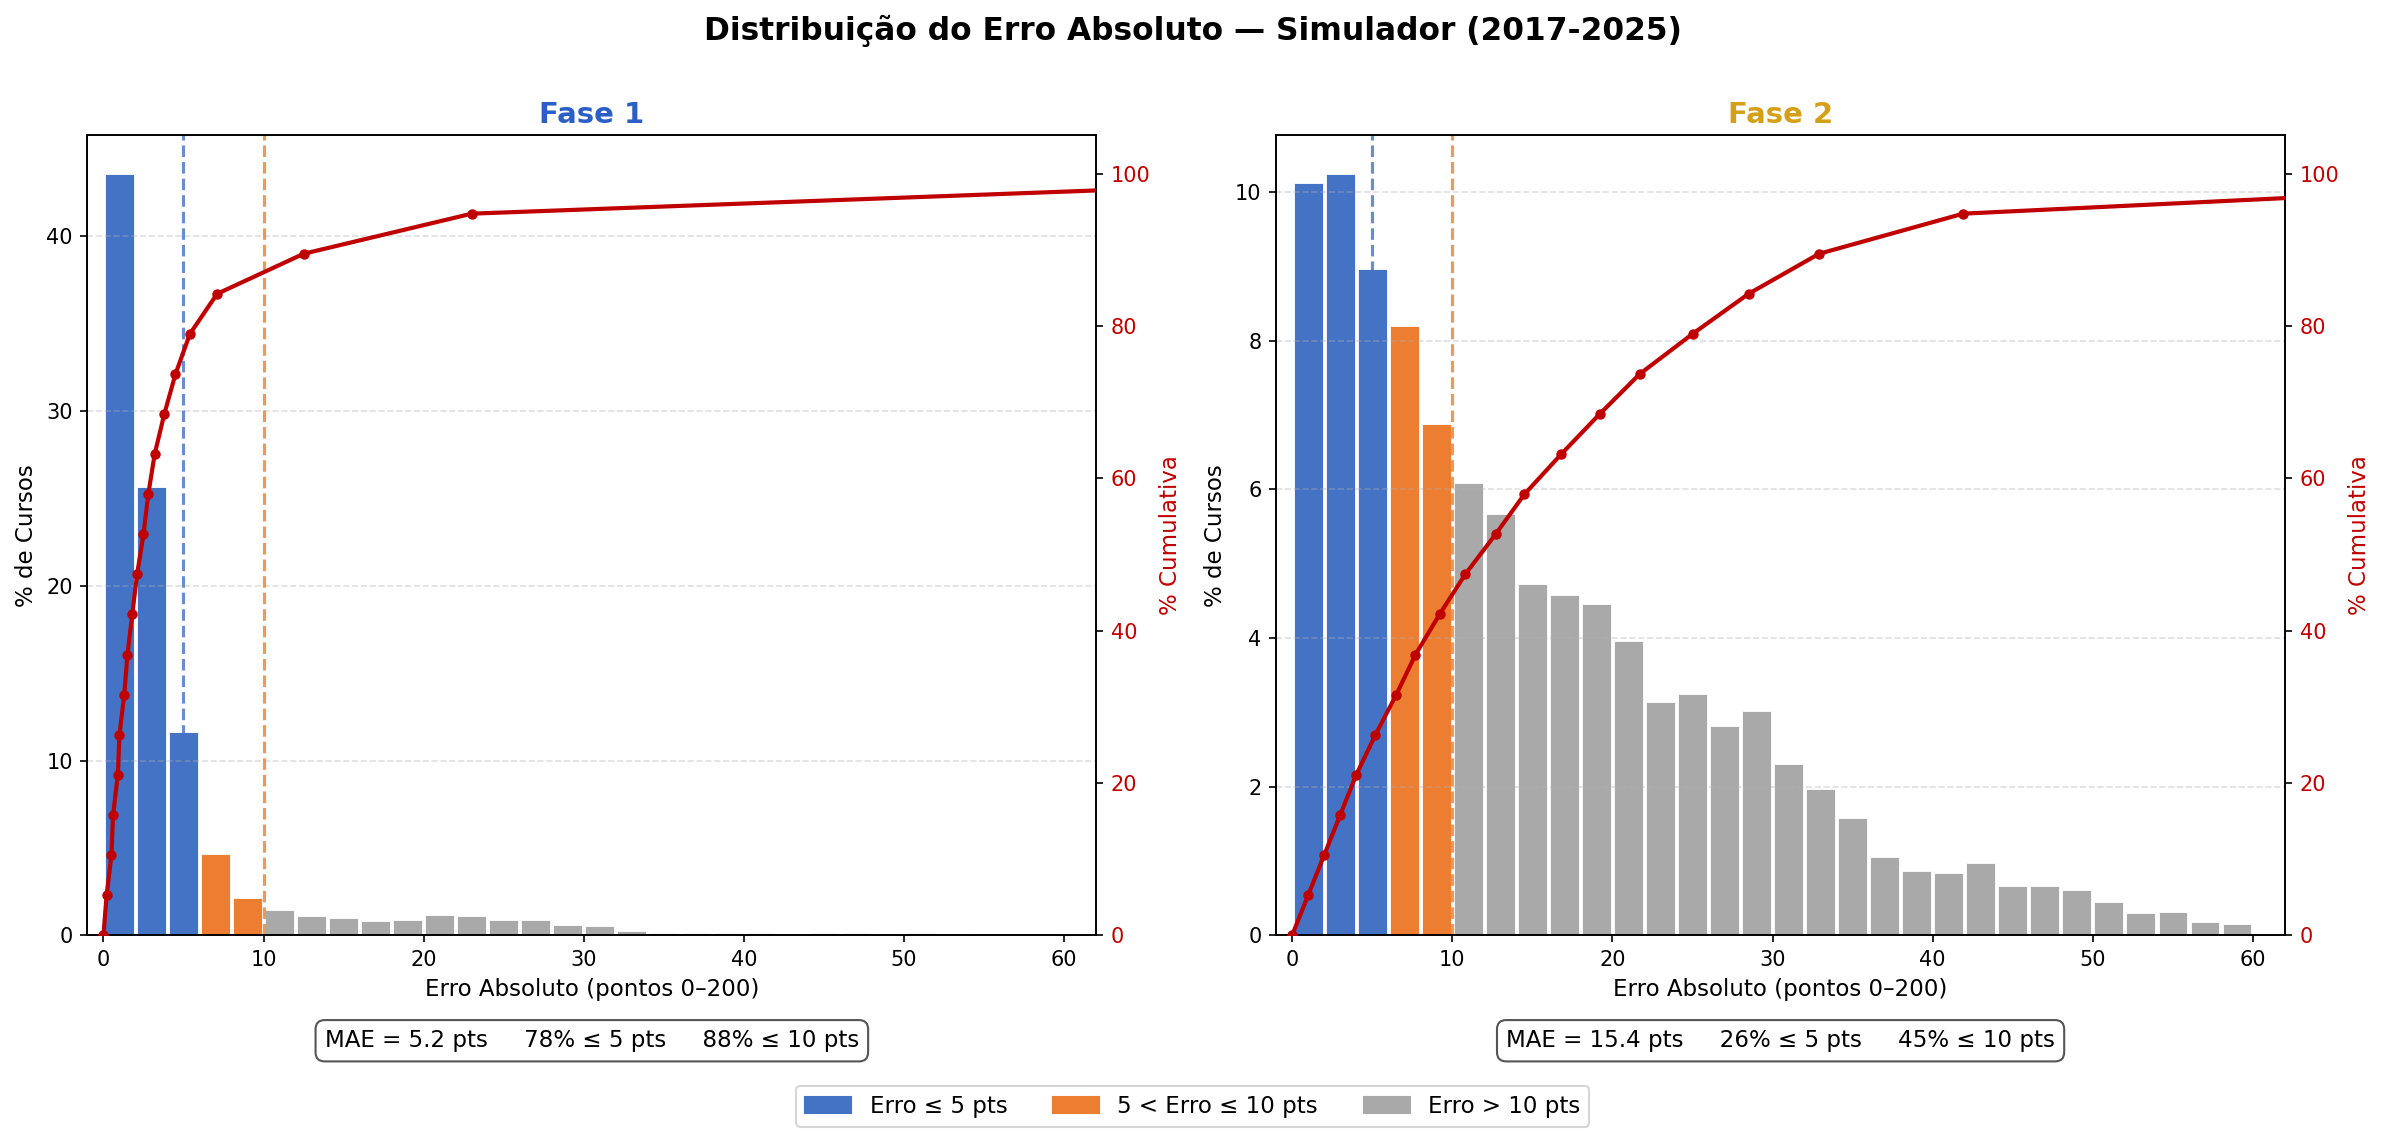
\includegraphics[width=\textwidth]{hist_erros.png}
  \caption{Distribuição do erro absoluto do motor de simulação para as Fases~1 e~2 (2017--2025).}
  \label{fig:hist_erros}
\end{figure}

Os resultados mostram que a Fase~1 é simulada com alta precisão: \textbf{MAE = 5.2 pontos} (escala 0--200), com 78\% dos cursos a apresentar erro inferior a 5 pontos e 88\% com erro inferior a 10 pontos. A Fase~2 é significativamente mais difícil de simular (MAE = 15.4 pontos), o que é esperado dado o menor volume de candidatos e a maior volatilidade das notas nesta fase.

A Figura~\ref{fig:mae_anual} mostra a evolução do MAE ao longo dos anos, revelando que a precisão na Fase~1 é estável (MAE médio = 5.24 pontos) e não é significativamente afetada pela pandemia de COVID-19, ao contrário da Fase~2 que evidencia um pico em 2020.

\begin{figure}[H]
  \centering
  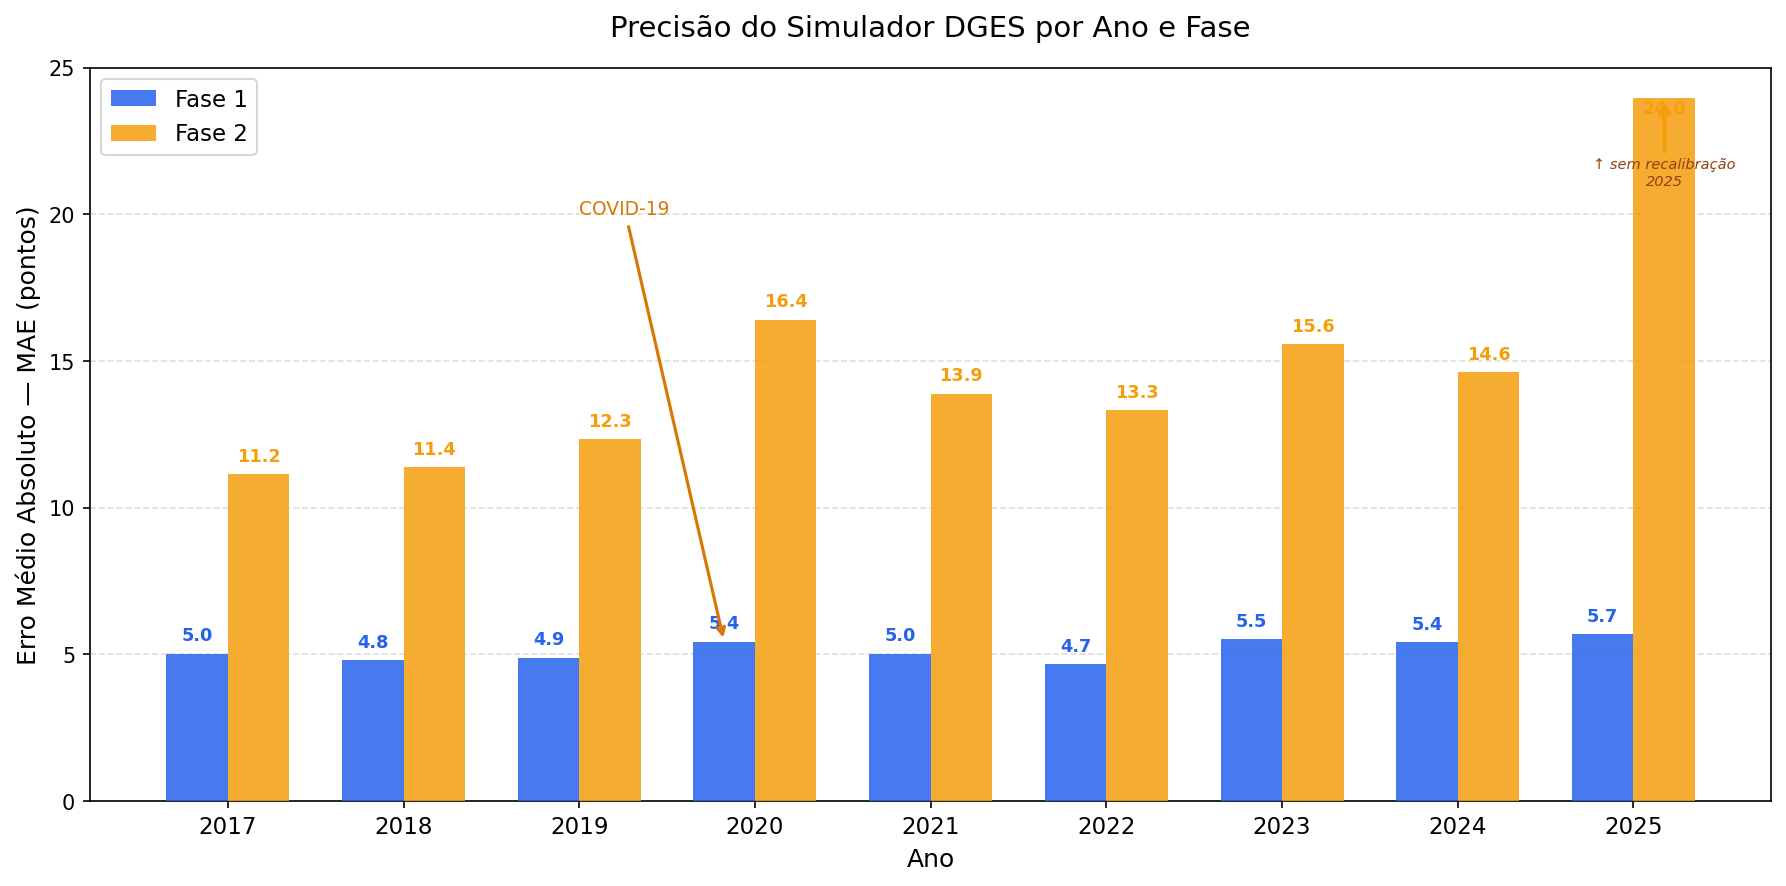
\includegraphics[width=\textwidth]{mae_por_ano.png}
  \caption{Evolução do MAE do simulador por ano para as Fases~1 e~2 (2017--2025).}
  \label{fig:mae_anual}
\end{figure}

A Figura~\ref{fig:scatter} ilustra a correlação entre notas reais e simuladas para o conjunto completo dos 9 anos, confirmando uma correlação linear forte na Fase~1 e maior dispersão na Fase~2.

\begin{figure}[H]
  \centering
  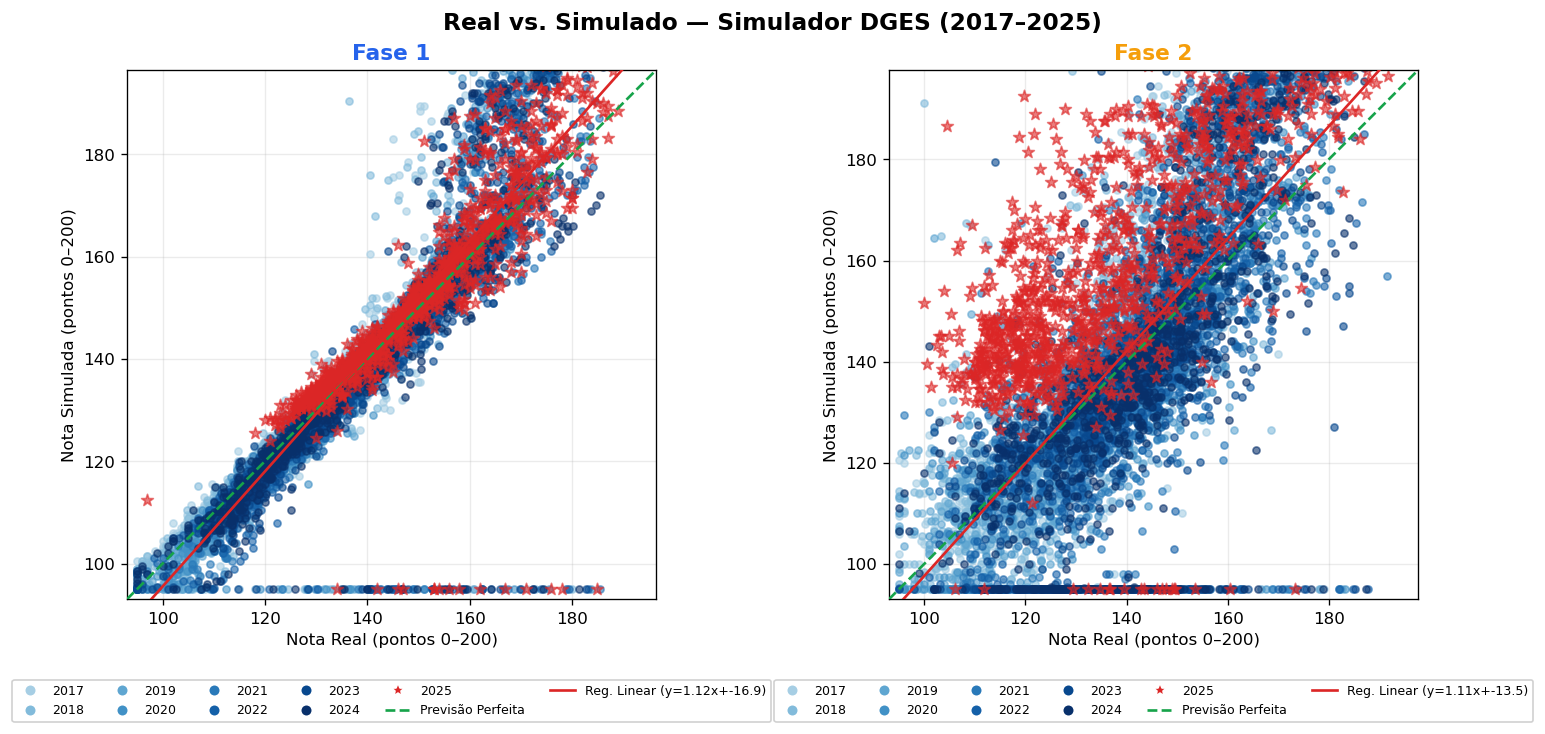
\includegraphics[width=0.85\textwidth]{scatter_real_vs_simulado.png}
  \caption{Correlação entre notas reais e simuladas para as Fases~1 e~2 (2017--2025).}
  \label{fig:scatter}
\end{figure}

\subsubsection{Validação do Algoritmo de Previsão}

O algoritmo de previsão foi validado por \textit{backtesting}: para cada ano de 2019 a 2024, o algoritmo foi alimentado com dados até ao ano anterior e a previsão foi comparada com os valores reais. A Figura~\ref{fig:previsao} mostra a distribuição do erro absoluto de previsão por ano.

\begin{figure}[H]
  \centering
  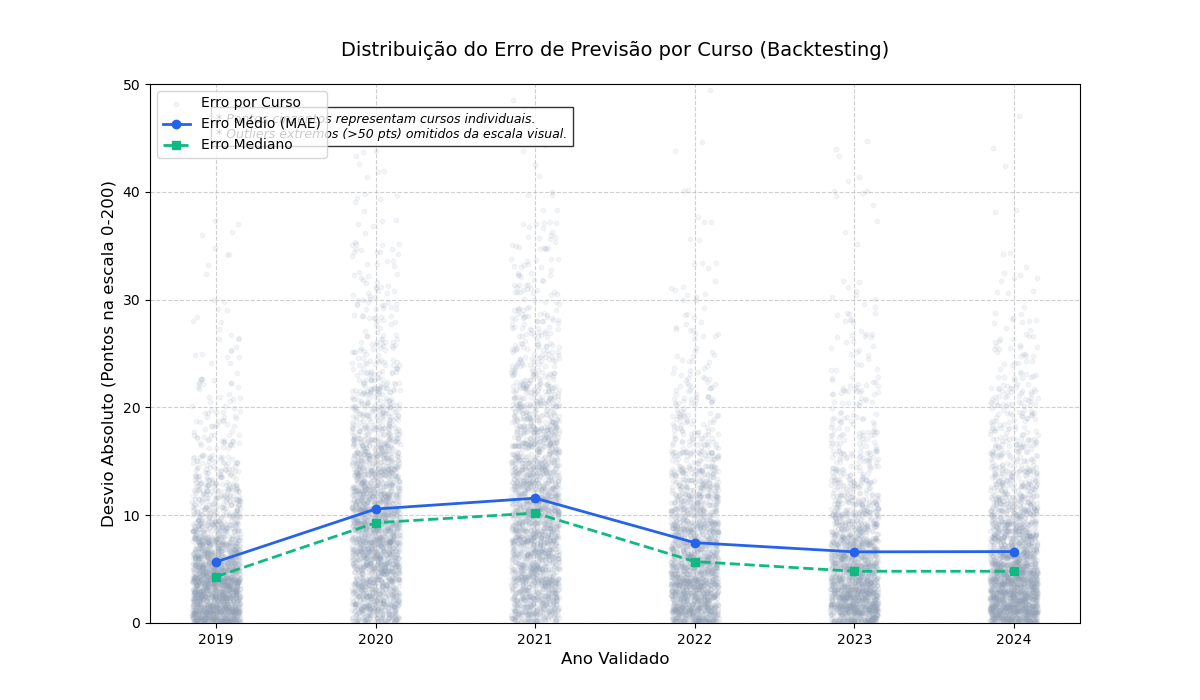
\includegraphics[width=0.7\textwidth]{desvio_previsoes_por_ano.png}
  \caption{Distribuição do erro de previsão por curso em \textit{backtesting} (2019--2024).}
  \label{fig:previsao}
\end{figure}

O MAE médio de previsão estabiliza em torno de \textbf{5--8 pontos} a partir de 2022. O pico de erro em 2020--2021 deve-se às anomalias introduzidas pela pandemia de COVID-19 nos resultados dos exames nacionais, que produziram uma inflação atípica das notas de acesso não prevista pelos dados históricos anteriores.

A Figura~\ref{fig:comparacao} apresenta a comparação entre o método de suavização exponencial simples e o sistema de simulação completo para previsão de notas (MAE global: 7.41~pts vs.\ 5.19~pts), evidenciando a vantagem do sistema de simulação baseado em IA para previsão.

\begin{figure}[H]
  \centering
  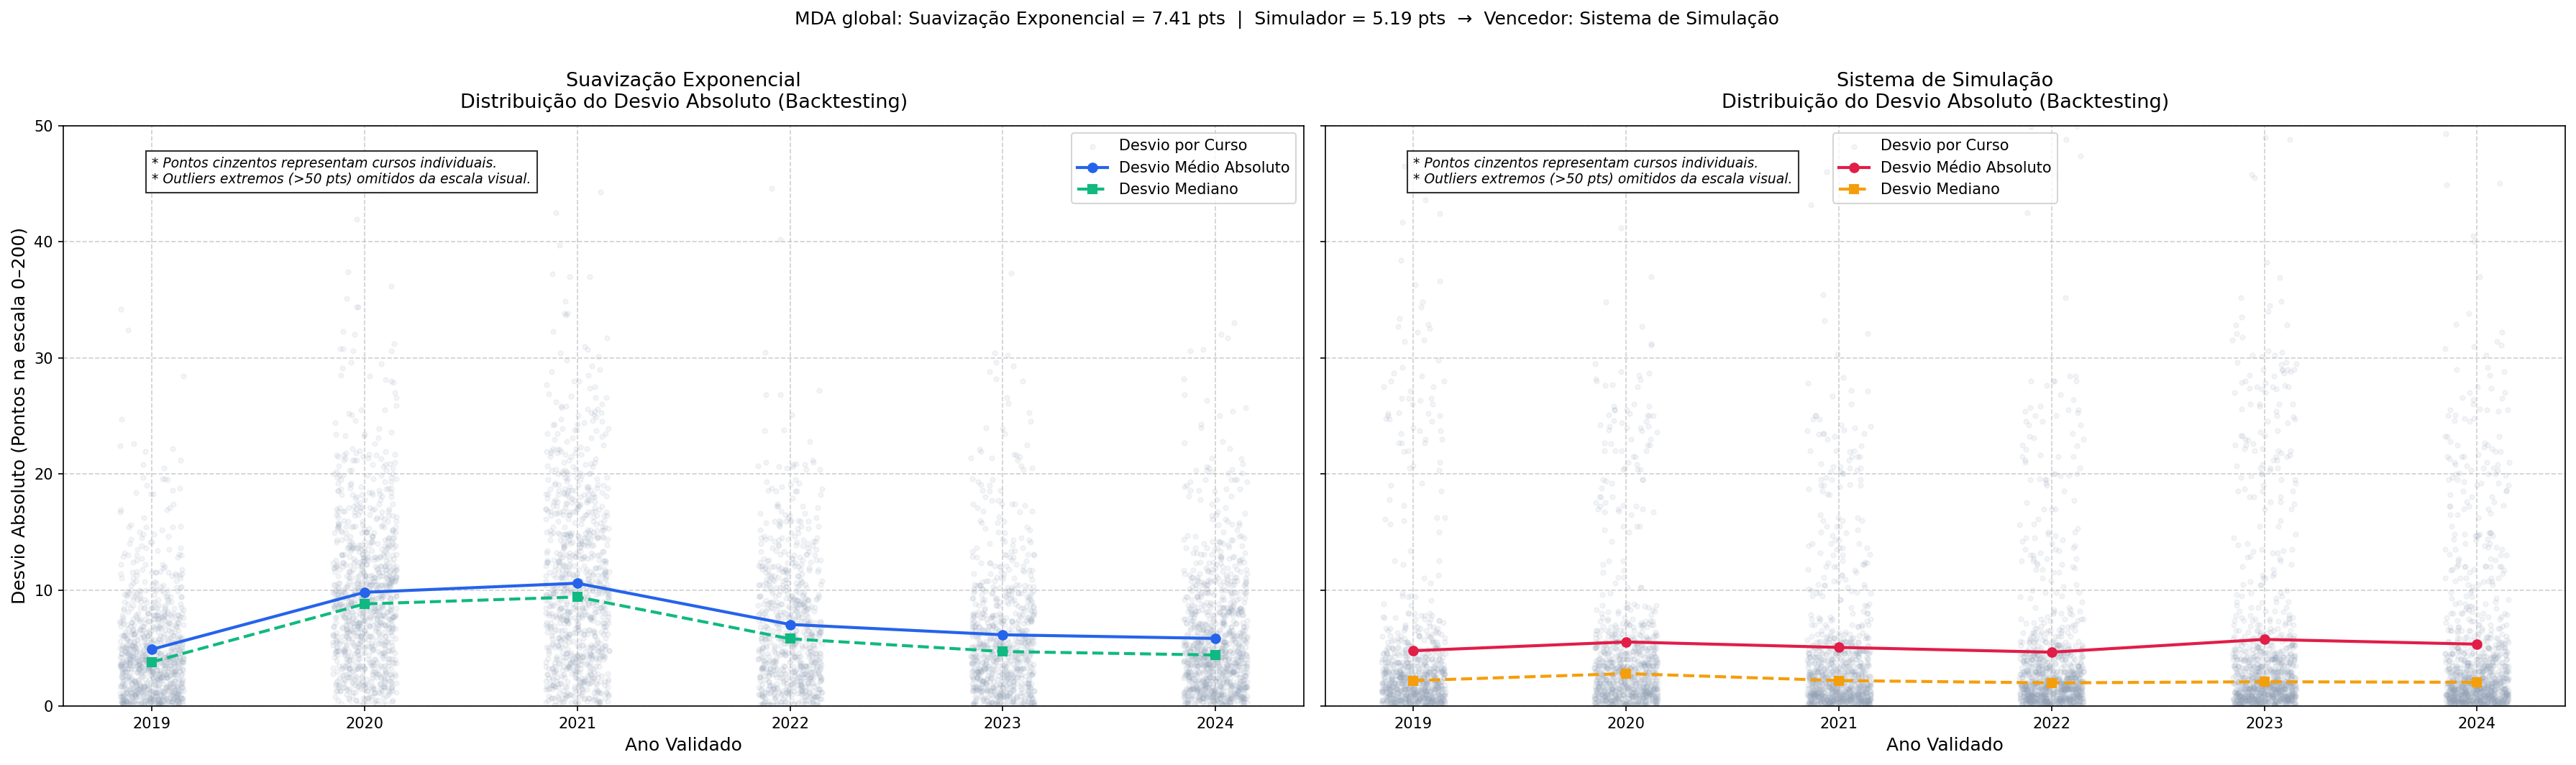
\includegraphics[width=\textwidth]{comparacao_simulador_vs_exp.png}
  \caption{Comparação entre suavização exponencial e o sistema de simulação em \textit{backtesting} (2019--2024).}
  \label{fig:comparacao}
\end{figure}

% ============================================================
% 4. CONCLUSÕES
% ============================================================
\section{Conclusões}
\label{sec:conclusoes}

\subsection{Resultados Alcançados}

O projeto MediaTrix cumpriu todos os objetivos definidos. Foram desenvolvidos e integrados com sucesso:

\begin{itemize}[noitemsep]
  \item Uma base de dados estruturada com informação de \textbf{1\,105 cursos} de \textbf{mais de 150 instituições} do ensino superior português, cobrindo \textbf{9 anos de dados} (2017--2025).
  \item Um motor de simulação do processo de candidatura com MAE de 5.2 pontos na Fase~1 (escala 0--200), utilizando geração de populações sintéticas e o algoritmo Gale-Shapley adaptado.
  \item Um modelo de IA treinado por \textit{online learning} com \textit{backpropagation} e \textit{momentum} ao longo de 9 anos, capaz de calibrar dinamicamente o comportamento de preferência dos candidatos.
  \item Um algoritmo de previsão com MAE de \textit{backtesting} de 5.19 pontos e intervalos de confiança de 95\%.
  \item Uma plataforma web completa e responsiva, integrando pesquisa de cursos, visualização histórica, previsões e simulador de candidatura.
\end{itemize}

O resultado superou o critério de qualidade inicial (erro médio inferior a 10 pontos) tanto na simulação da Fase~1 como na previsão.

\subsection{Contribuições Individuais}

O projeto foi desenvolvido por uma equipa de quatro elementos, sob orientação do Prof.\ Carlos Baquero. As contribuições individuais são descritas na Tabela~\ref{tab:contribuicoes}.

\begin{table}[H]
\centering
\caption{Contribuições individuais dos membros da equipa.}
\label{tab:contribuicoes}
\begin{tabularx}{\textwidth}{llXr}
\toprule
\textbf{Elemento} & \textbf{Número} & \textbf{Contribuição Principal} & \textbf{\%} \\
\midrule
José Torres   & up202307047 &  & \% \\
José Reis     & up202307304 &  & \% \\
Tiago Yin     & up202306438 &  & \% \\
Vicente Silva & up202303702  &  & \% \\
\bottomrule
\end{tabularx}
\end{table}

\subsection{Lições Aprendidas}

O projeto proporcionou aprendizagens significativas em diversas dimensões dos objetivos de aprendizagem da UC:

\begin{itemize}
  \item \textbf{Engenharia de dados e qualidade dos dados (A)}: a recolha e estruturação de dados heterogéneos provenientes de relatórios DGES, DGEEC e estatísticas de exames revelou-se uma tarefa morosa e crítica para a qualidade de todo o sistema a jusante.

  \item \textbf{Modelação de sistemas sociais complexos (A)}: simular o comportamento de 75\,000 candidatos num mercado dinâmico exige decisões de modelação cuidadas. O choque pandémico de 2020 revelou os limites de modelos estocásticos face a perturbações sistémicas não observadas no histórico de treino.

  \item \textbf{Equilíbrio entre complexidade e precisão (A)}: a comparação entre o método de suavização exponencial e o simulador completo mostrou que a escolha do método deve ser guiada por validação empírica e não por intuição sobre a complexidade do modelo.

  \item \textbf{Comunicação de incerteza (D)}: a apresentação de intervalos de confiança em vez de valores pontuais requer cuidados na interface. A inclusão de uma secção de ``Limitações'' foi essencial para que os utilizadores interpretem as previsões de forma correta e responsável.

  \item \textbf{Desenvolvimento \textit{frontend} moderno (A, D)}: o ecossistema React + TypeScript + Vite revelou-se produtivo, com curva de aprendizagem relevante na gestão de estado assíncrono, na otimização de re-renderizações com \textit{memoization} e no \textit{design} responsivo.
\end{itemize}

\subsection{Limitações e Trabalho Futuro}

As principais limitações do trabalho são:

\begin{itemize}[noitemsep]
  \item O modelo não integra variáveis exógenas como o número previsível de candidatos no ano seguinte ou os resultados preliminares dos exames nacionais, que poderiam melhorar a precisão das previsões.
  \item A Fase~2 e a Fase~3 apresentam maior erro de simulação, em parte porque os candidatos destas fases têm comportamentos mais difíceis de modelar com populações sintéticas de dimensão fixa.
  \item A recolha de dados DGES é manual, tornando a atualização anual dependente da disponibilidade da equipa.
\end{itemize}

O trabalho futuro inclui:

\begin{enumerate}[noitemsep]
  \item Automatização da recolha de dados DGES através de \textit{web scraping}.
  \item Integração de dados de exames nacionais em tempo real para refinar as previsões à medida que os resultados são publicados.
  \item Exploração de modelos de séries temporais mais sofisticados (ARIMA, Prophet~\cite{taylor2018forecasting}) para comparação com a abordagem atual.
  \item Adição de funcionalidades de alerta (por correio eletrónico) quando as previsões de um curso atingem um determinado limiar.
  \item Publicação da plataforma em produção (\textit{deploy} em Vercel ou Netlify).
\end{enumerate}

\subsection{Contribuição para os Objetivos de Desenvolvimento Sustentável}

O MediaTrix contribui para o \textbf{ODS~4 --- Educação de Qualidade}~\cite{sdgs}, ao democratizar o acesso a informação quantitativa e fundamentada sobre as notas de acesso ao ensino superior. Ao reduzir a incerteza no processo de candidatura, a plataforma pode ajudar candidatos de contextos socioeconómicos menos favorecidos --- que têm tipicamente menos acesso a orientação vocacional profissional --- a tomar decisões mais informadas. Contribui assim também, de forma indireta, para o \textbf{ODS~10 --- Redução das Desigualdades}, ao nivelar o acesso à informação independentemente da capacidade financeira de contratar apoio especializado.

% ============================================================
% REFERÊNCIAS
% ============================================================
\bibliographystyle{plain}
\bibliography{references}

\end{document}
